\section{Android-Messungen
\label{section:androidmeasurements}}
Nachfolgend sind die Messungen auf Mobilgeräten mit Android-Betriebs-systemen 
und daraus gewonnene Erkenntnisse beschrieben.

Gesamthaft wurden 70 Einzelmessungen in 28 Stunden und 40 Minuten durchgeführt.

\subsection{Versuchsdurchführung}
Die im Unterabschnitt~\ref{subsection:plannedexperiments} genannten
Messungen wurden auf insgesamt neun Android-Geräten durchgeführt, welche in der 
Tabelle~\ref{table:measuredandroiddevices} aufgeführt werden.

\begin{table}[h!]
	\centering
	\begin{tabular}{|c|c|c|}
		\hline
        \textbf{Gerätetyp} & \textbf{Android-Version} & \textbf{Besitzer} \\
        \hline
        Samsung A51 & Android 10 & Janik Schlatter \\
        Fairphone 3+ & Android 10 & Mike Schmid \\
        Samsung Galaxy S8 & Android 9 & IFS \\
        Samsung Galaxy S8 & Android 9 & IFS \\
        Samsung Galaxy S8 & Android 9 & Janik Schlatter \\
        Samsung Galaxy S8 & Android 9 & Jenny Bösch \\
        Samsung Galaxy S9 & Android 10 & IFS \\
        Samsung Galaxy S20+ &  Android 10 & IFS \\
        Google Pixel 3  & Android 11 & IFS \\
        \hline
    \end{tabular}
    \caption{Gemessene Android-Geräte
    \label{table:measuredandroiddevices}}  
\end{table}

Die Messungen auf allen Geräten ausser den vier Galaxy S8 Geräten wurden komplett
durchgeführt. Die S8 mit Android 9 verschleiern ihre MAC-Adresse in Probe-Requests
nicht, weswegen auf diesen vier Geräten nur 20-minütige Aktivtests durchgeführt
wurden. 

Weiterhin stand für die zweite Woche in den Android-Messungen der Wave-Xpert, 
ein WLAN-Messgerät mit dem mehrere Kanäle gleichzeitig gemessen werden können,
zur Verfügung. Mit dem WaveXpert wurden die Messungen mit dem Fairphone 3+ und 
Messungen mit mehreren parallel laufenden Geräten durchgeführt.
Diese parallelen Messungen dienen der Verifikation eines Prototypen mit Daten, 
die ein realistischeres Umfeld darstellen, deren Parameter (Anzahl Geräte, 
Laufzeit, welche Geräte verbunden sind, etc.) aber beeinflusst werden können.

\subsection{Ergebnisse}
Die folgenden Messergebnisse konnten in den Messungen produziert werden.

\subsubsection*{Probe-Requests}
In der Tabelle~\ref{table:androidproberesults} ist ersichtlich, wie viele Probe 
Requests pro Messung aufgezeichnet wurden, wie viele davon in Bursts gruppiert
waren, die minimale, durchschnittliche und maximale Burstgrösse sowie eine 
Schätzung der nicht aufgezeichneten Frames und die durchschnittliche 
Zwischenankunftszeit zwischen zwei Bursts.

\begin{landscape}
    \begin{table}[h!]
        \small
	    \centering
        \begin{tabular}{|c|c|c|c|c|c|c|c|c|}
            \hline
            \textbf{Gerät} & \textbf{Android}  & \textbf{Anzahl} & \textbf{Anzahl} & \textbf{min.} & \textbf{avg.} & \textbf{max.} & \textbf{Verpasste} & \textbf{Zwischen-}\\
             & \textbf{Version} & \textbf{Probe-Requests} & \textbf{Bursts} & \textbf{Burstgrösse} & \textbf{Burstgrösse} & \textbf{Burstgrösse} & \textbf{Frames} & \textbf{ankunftszeit}\\
            \hline
            \shortstack{Samsung \\ A51 } &  10 & \phantom{0}412 & \phantom{00}61 & 2 & \phantom{0}6,409 & 12 & \phantom{0}270 & 276,04 s \\
            \hline
            \shortstack{Samsung \\ Galaxy S9 } &  10 & \phantom{0}384 & \phantom{0}125 & 1 & \phantom{0}2,897 & \phantom{0}7 & \phantom{0}632 & 211,88 s \\
            \hline
            \shortstack{Samsung \\ Galaxy S20+ } &  10 & \phantom{0}489 & \phantom{0}303 & 1 & \phantom{0}1,889 & \phantom{0}2 & \phantom{0}161 & 118,00 s \\
            \hline
            \shortstack{Google \\ Pixel 3 } &  11 & 5048 & \phantom{0}960 & 1 & \phantom{0}4,415 & 15 & 2076 & 32,99 s \\
            \hline
            \shortstack{Samsung \\ Galaxy S8 } & \phantom{0}9 & \phantom{00}44 &\phantom{00} 12 & 2 & \phantom{0}3,667 & \phantom{0}6 & \phantom{00}32 & \phantom{0}94,27 s \\
            \hline
            \shortstack{Samsung \\ Galaxy S8 } &  \phantom{0}9 & \phantom{00}60 & \phantom{00}11 & 2 & \phantom{0}5,455 & 10 & \phantom{00}64 & 101,21 s \\
            \hline
            \shortstack{Samsung \\ Galaxy S8 } &  \phantom{0}9 & \phantom{0}149 & \phantom{00}20 & 1 & \phantom{0}7,450 & 13 & \phantom{0}149 & \phantom{0}55,78 s \\
            \hline
            \shortstack{Samsung \\ Galaxy S8 } &  \phantom{0}9 & \phantom{0}101 & \phantom{00}14 & 4 & \phantom{0}7,214 & 11 & \phantom{0}200 & \phantom{0}80,29 s \\
            \hline
            Fairphone 3+ &  10 & 2329 & \phantom{0}386 & 1 & 10,283 & 25 & \phantom{0}744 & \phantom{0}93,69 s \\
            \hline
            TOTAL & & 9016 & 1892 & 1 & \phantom{0}5,520 & 25 & 4328 & 118,24 s \\
            \hline
        \end{tabular}
        \caption{Ergebnisse der Android-Messungen
        \label{table:androidproberesults}}  
    \end{table}
    Die genauen Auswertungen der Messergebnisse finden sich im 
    Anhang~\ref{chapter:appendix:experimentaldata}. 
    Die Daten sind auf dem Repository im Ordner "Experimente" in den jeweiligen Unterordnern
    zu finden.

    \clearpage

    Nachfolgend sind in den Abbildungen die Graphische Auswertung nach Gesamtzahl
    (Abbildung~\ref{figure:totalandroidmeasurements}) der Messwerte und die Messergebnisse nach Kategorie für
    die einzelnen Android-Geräte (Abbildungen~\ref{figure:androidmeasurementsbycategorys8}
    bis~\ref{figure:androidmeasurementsbycategorypixel}) dargestellt.

    \begin{figure}[h!]
        \centering
        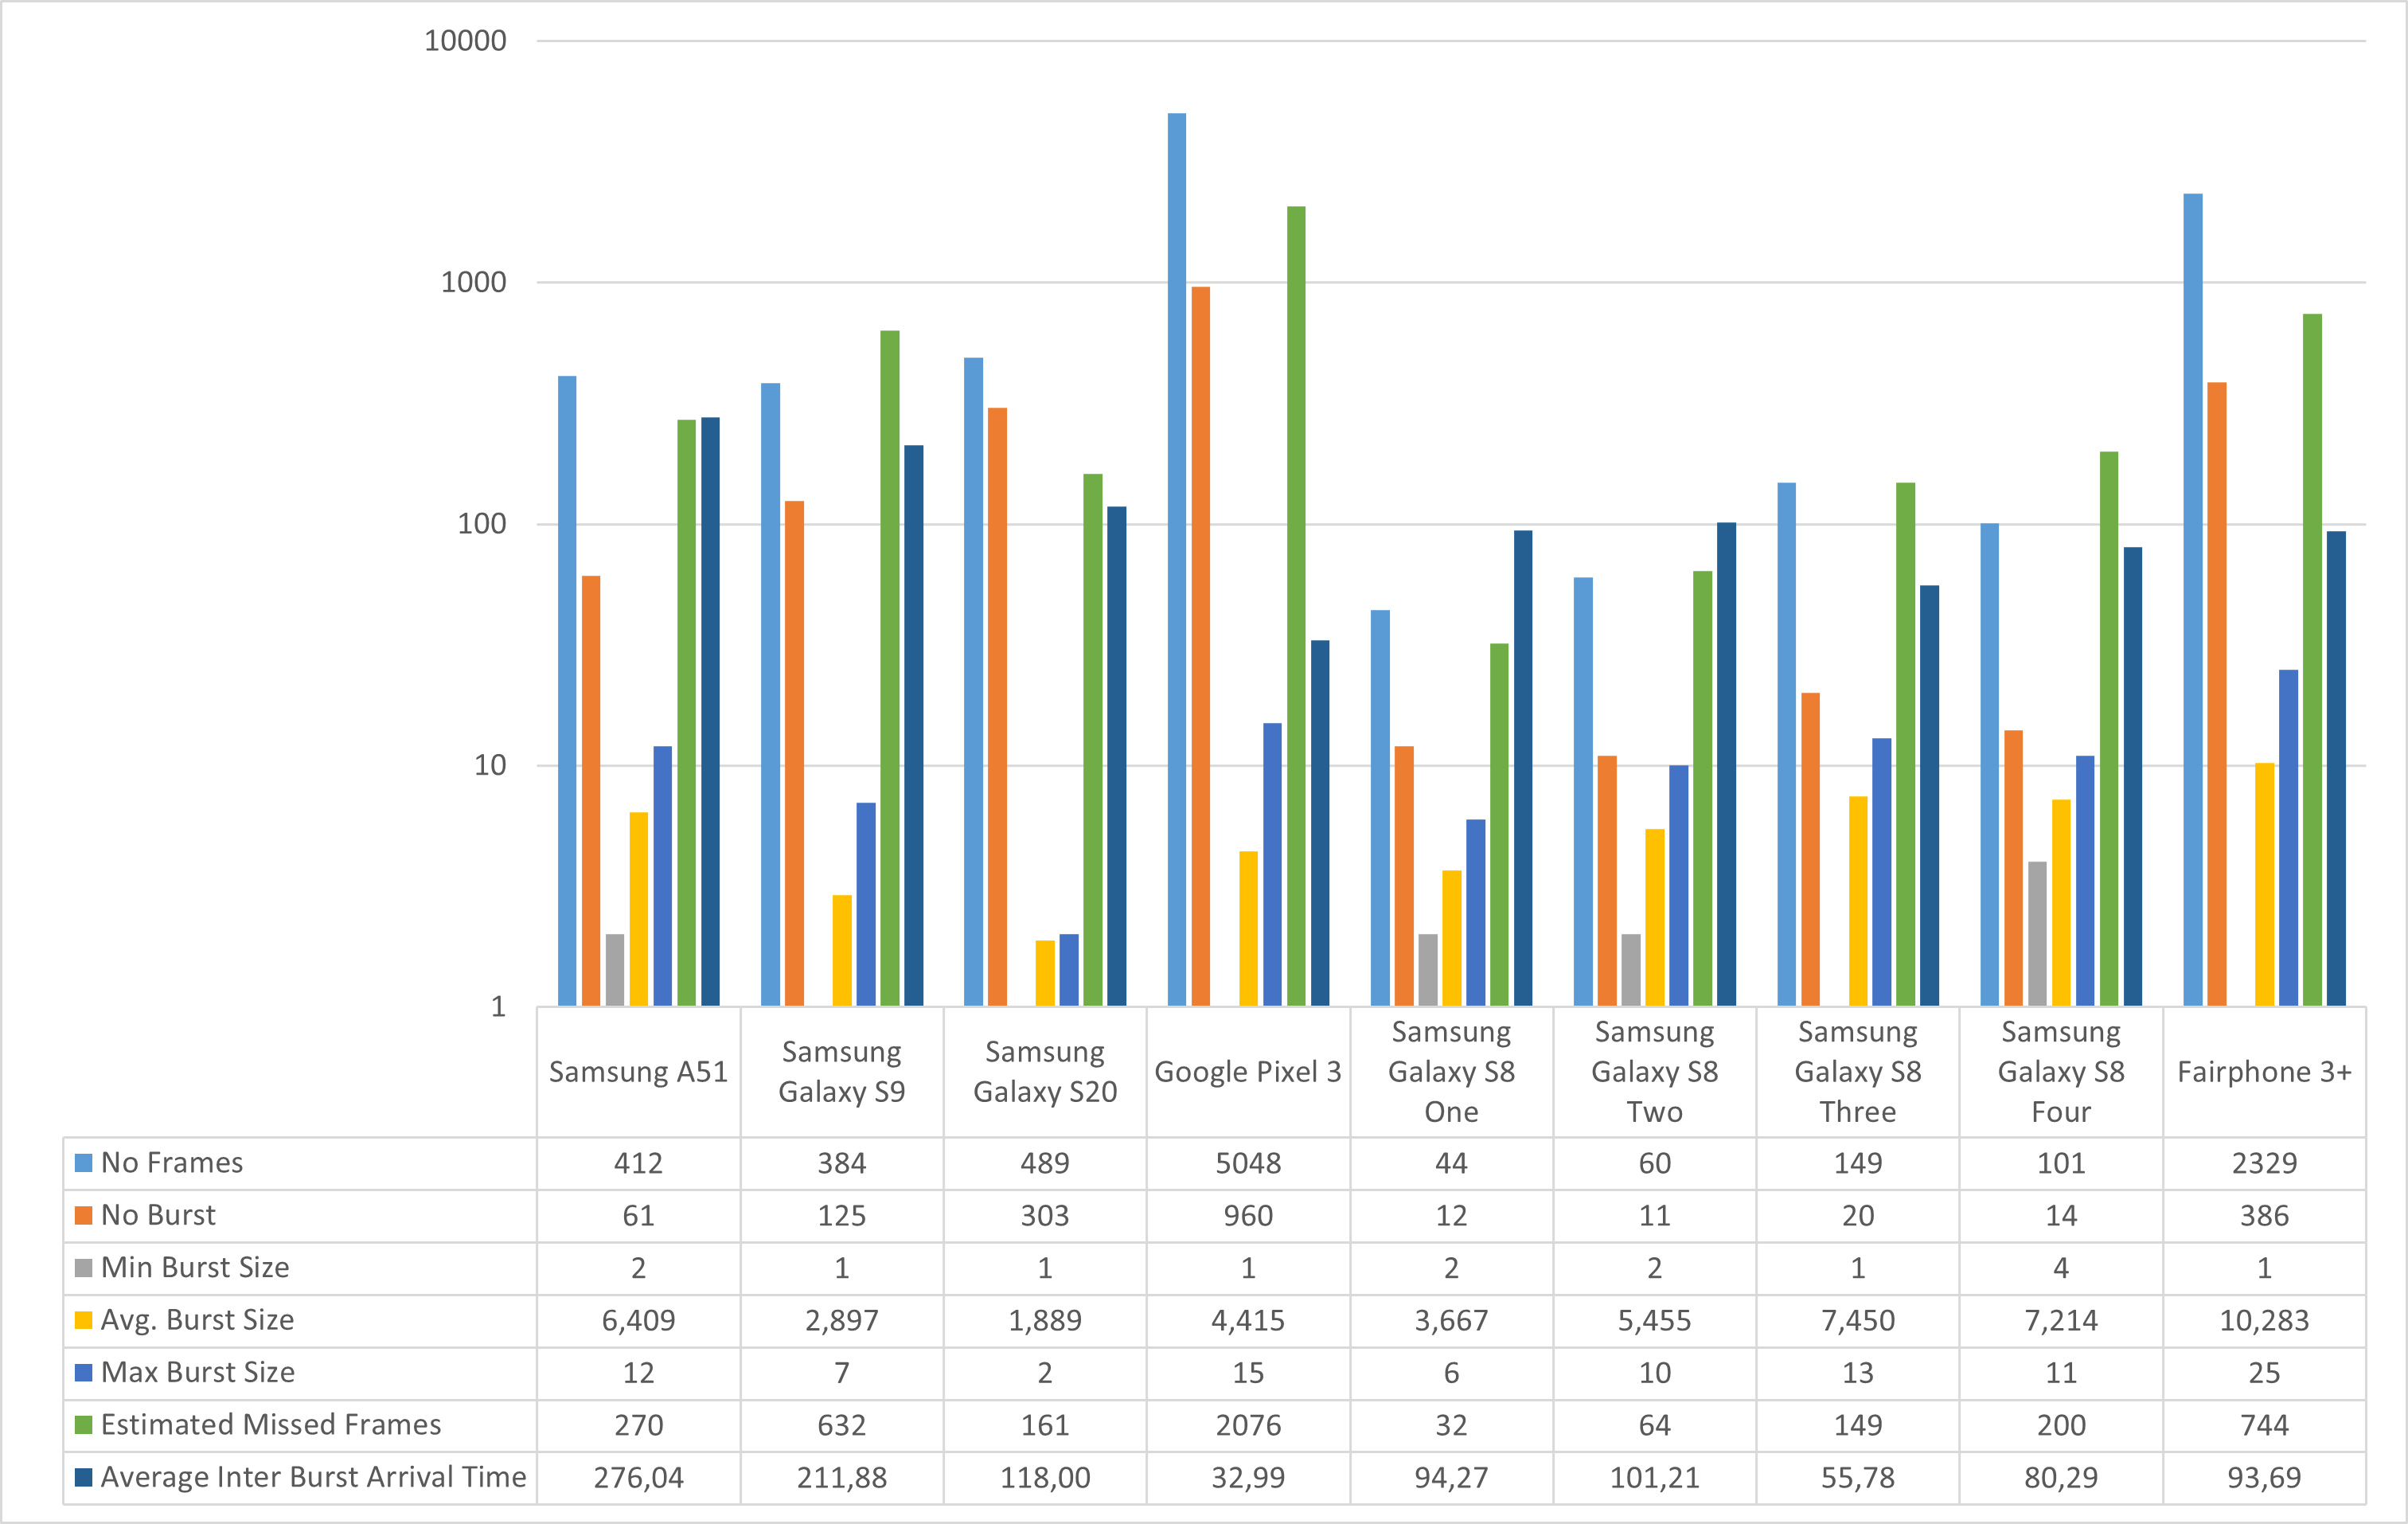
\includegraphics[width=0.75\linewidth]{Experiments/Android-Total.png}
        \caption{Gesamtergebnis der Android-Messungen}
        \label{figure:totalandroidmeasurements}
    \end{figure}
\end{landscape}

\clearpage

\begin{figure}[h!]
    \centering
    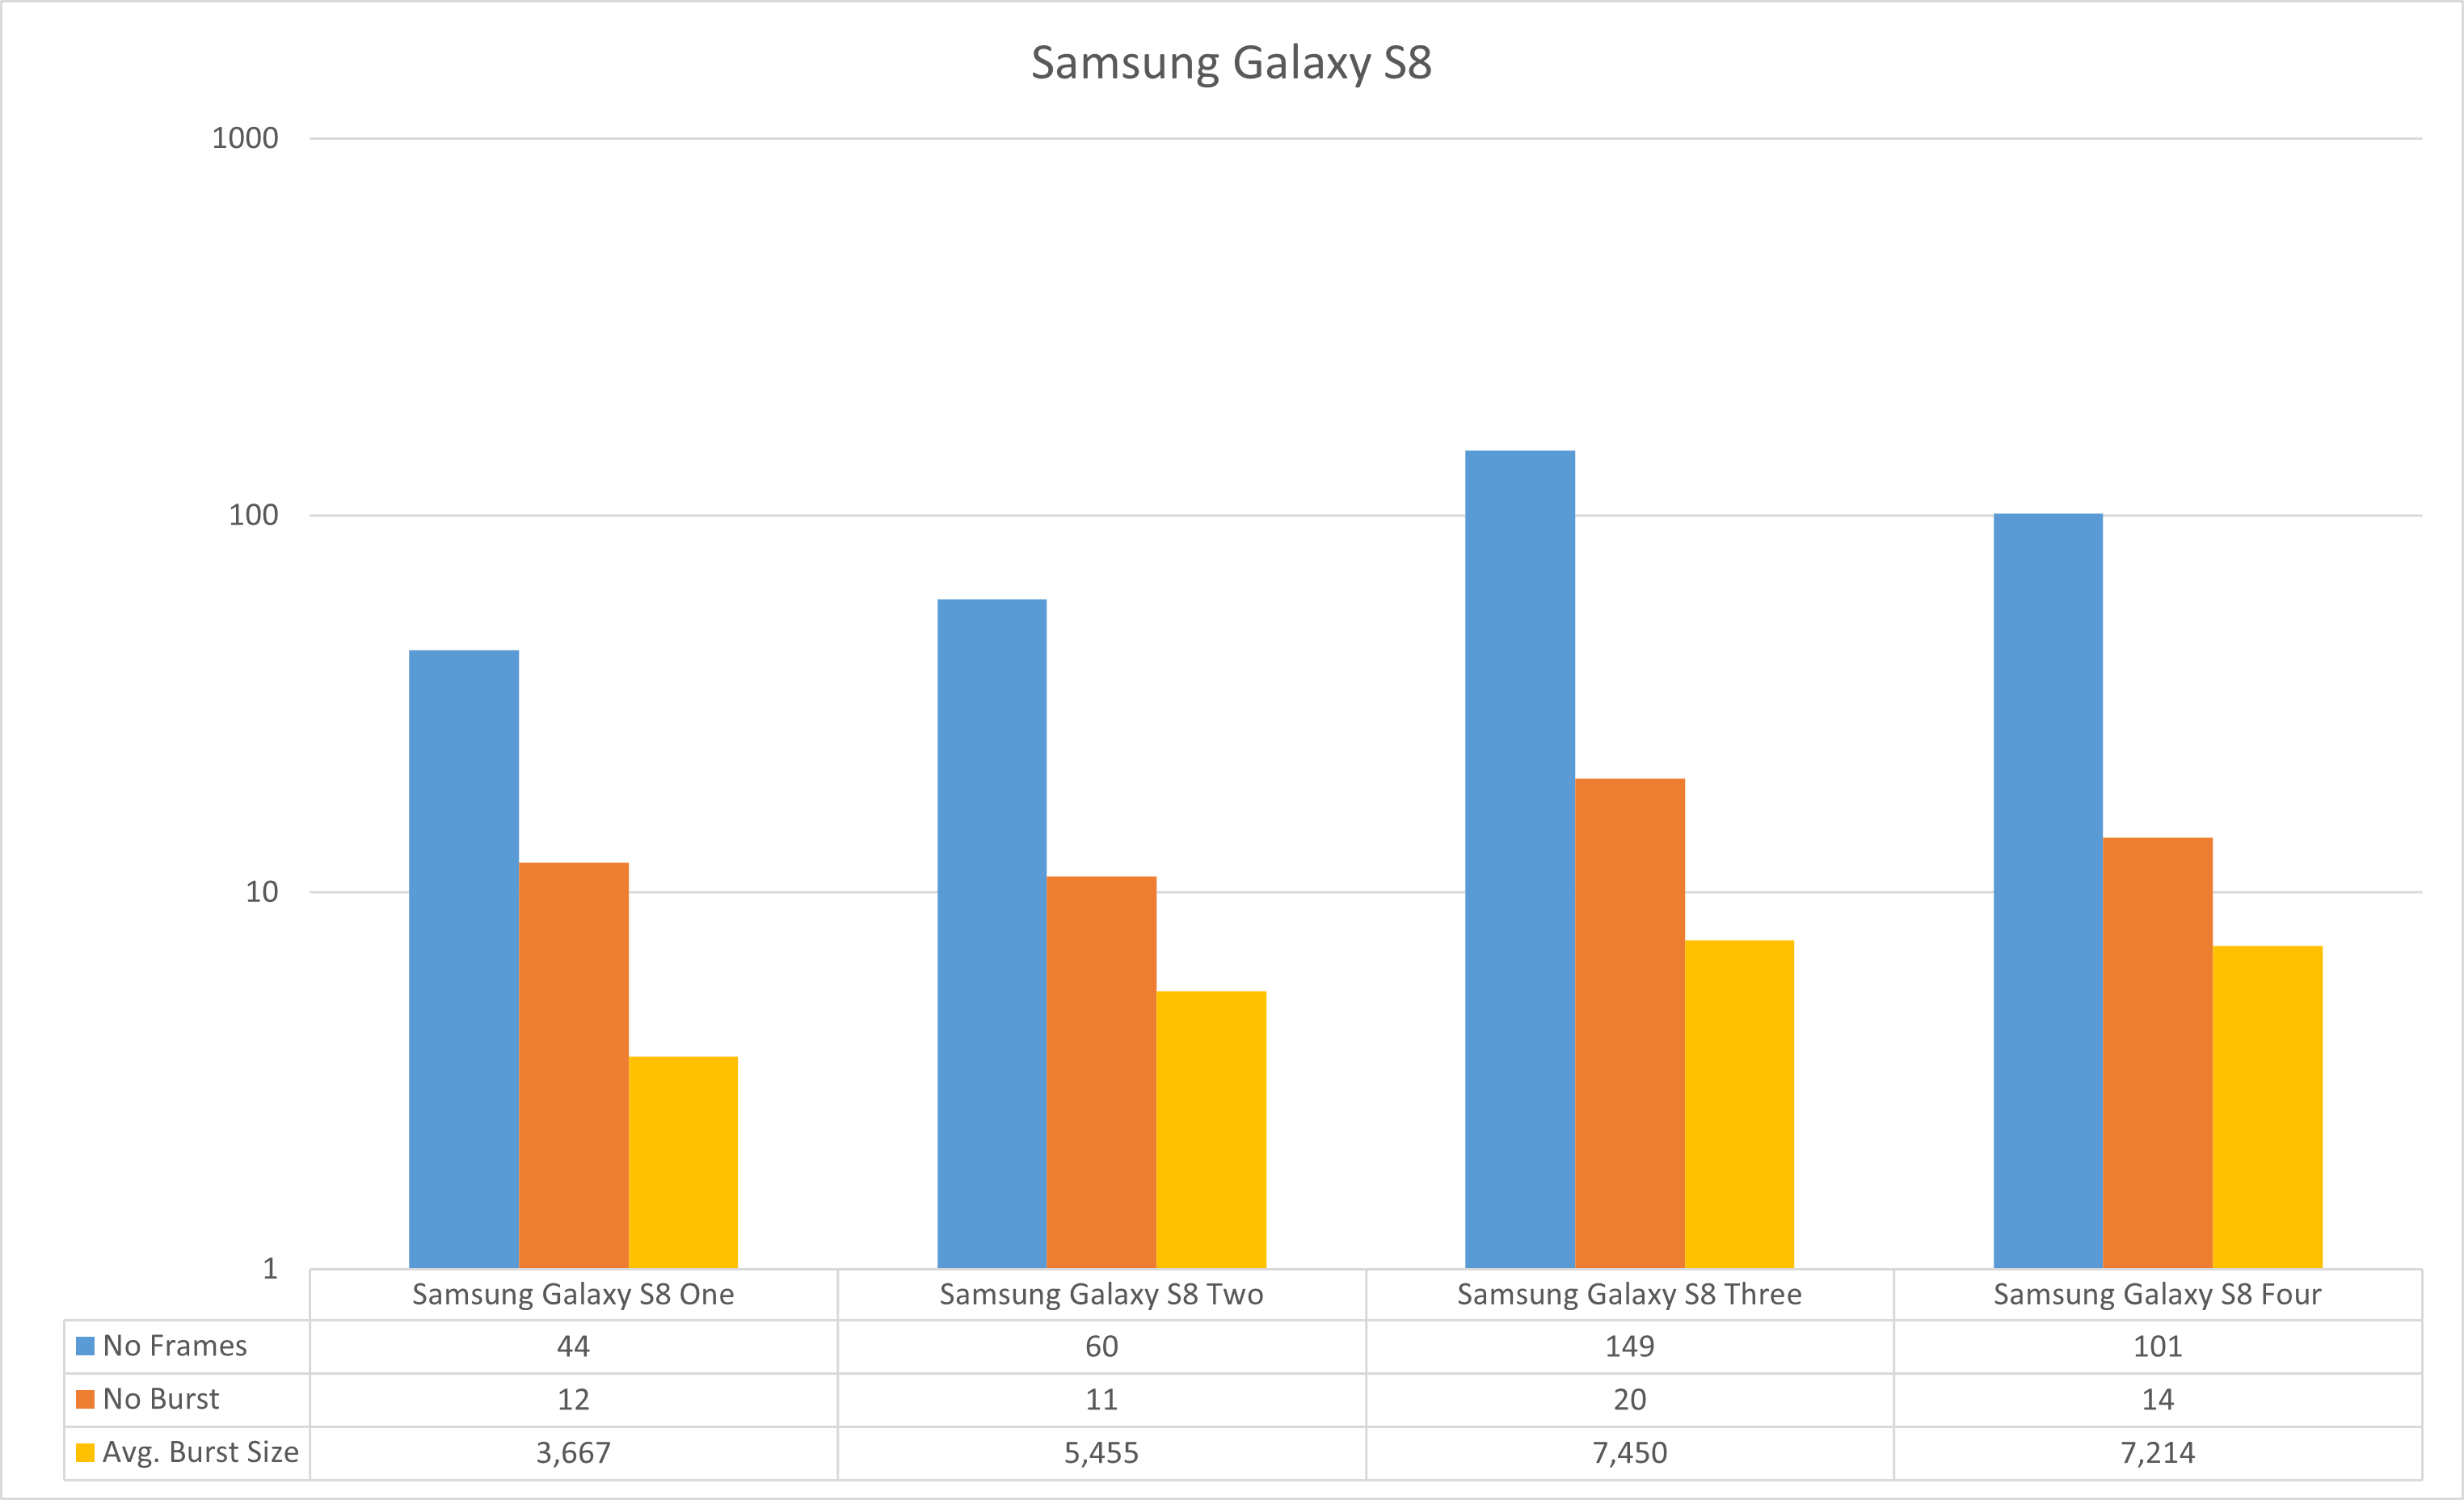
\includegraphics[width=1\linewidth]{Experiments/S8-Gruppe.png}
    \caption{Messergebnisse der vier Samsung Galaxy S8-Geräte mit Android 9}
    \label{figure:androidmeasurementsbycategorys8}
\end{figure}

In den Messungen der Samsung Galaxy S8 ist aufgefallen, dass diese bei 
Probe-Requests ihre echte Gerätemacadresse verwenden. Dieses Verhalten ist bei 
allen vier Geräten ersichtlich und lässt darauf schliessen, dass alle Samsung 
Galaxy Geräte der S8-Generation mit Android die MAC-Adresse nicht verschleiern.
(Sofern nicht über den Developermodus die seit Android 6 verfügbare Option 
gesetzt wurde, die MAC-Adressen zu randomisieren)

\clearpage

\begin{figure}[h!]
    \centering
    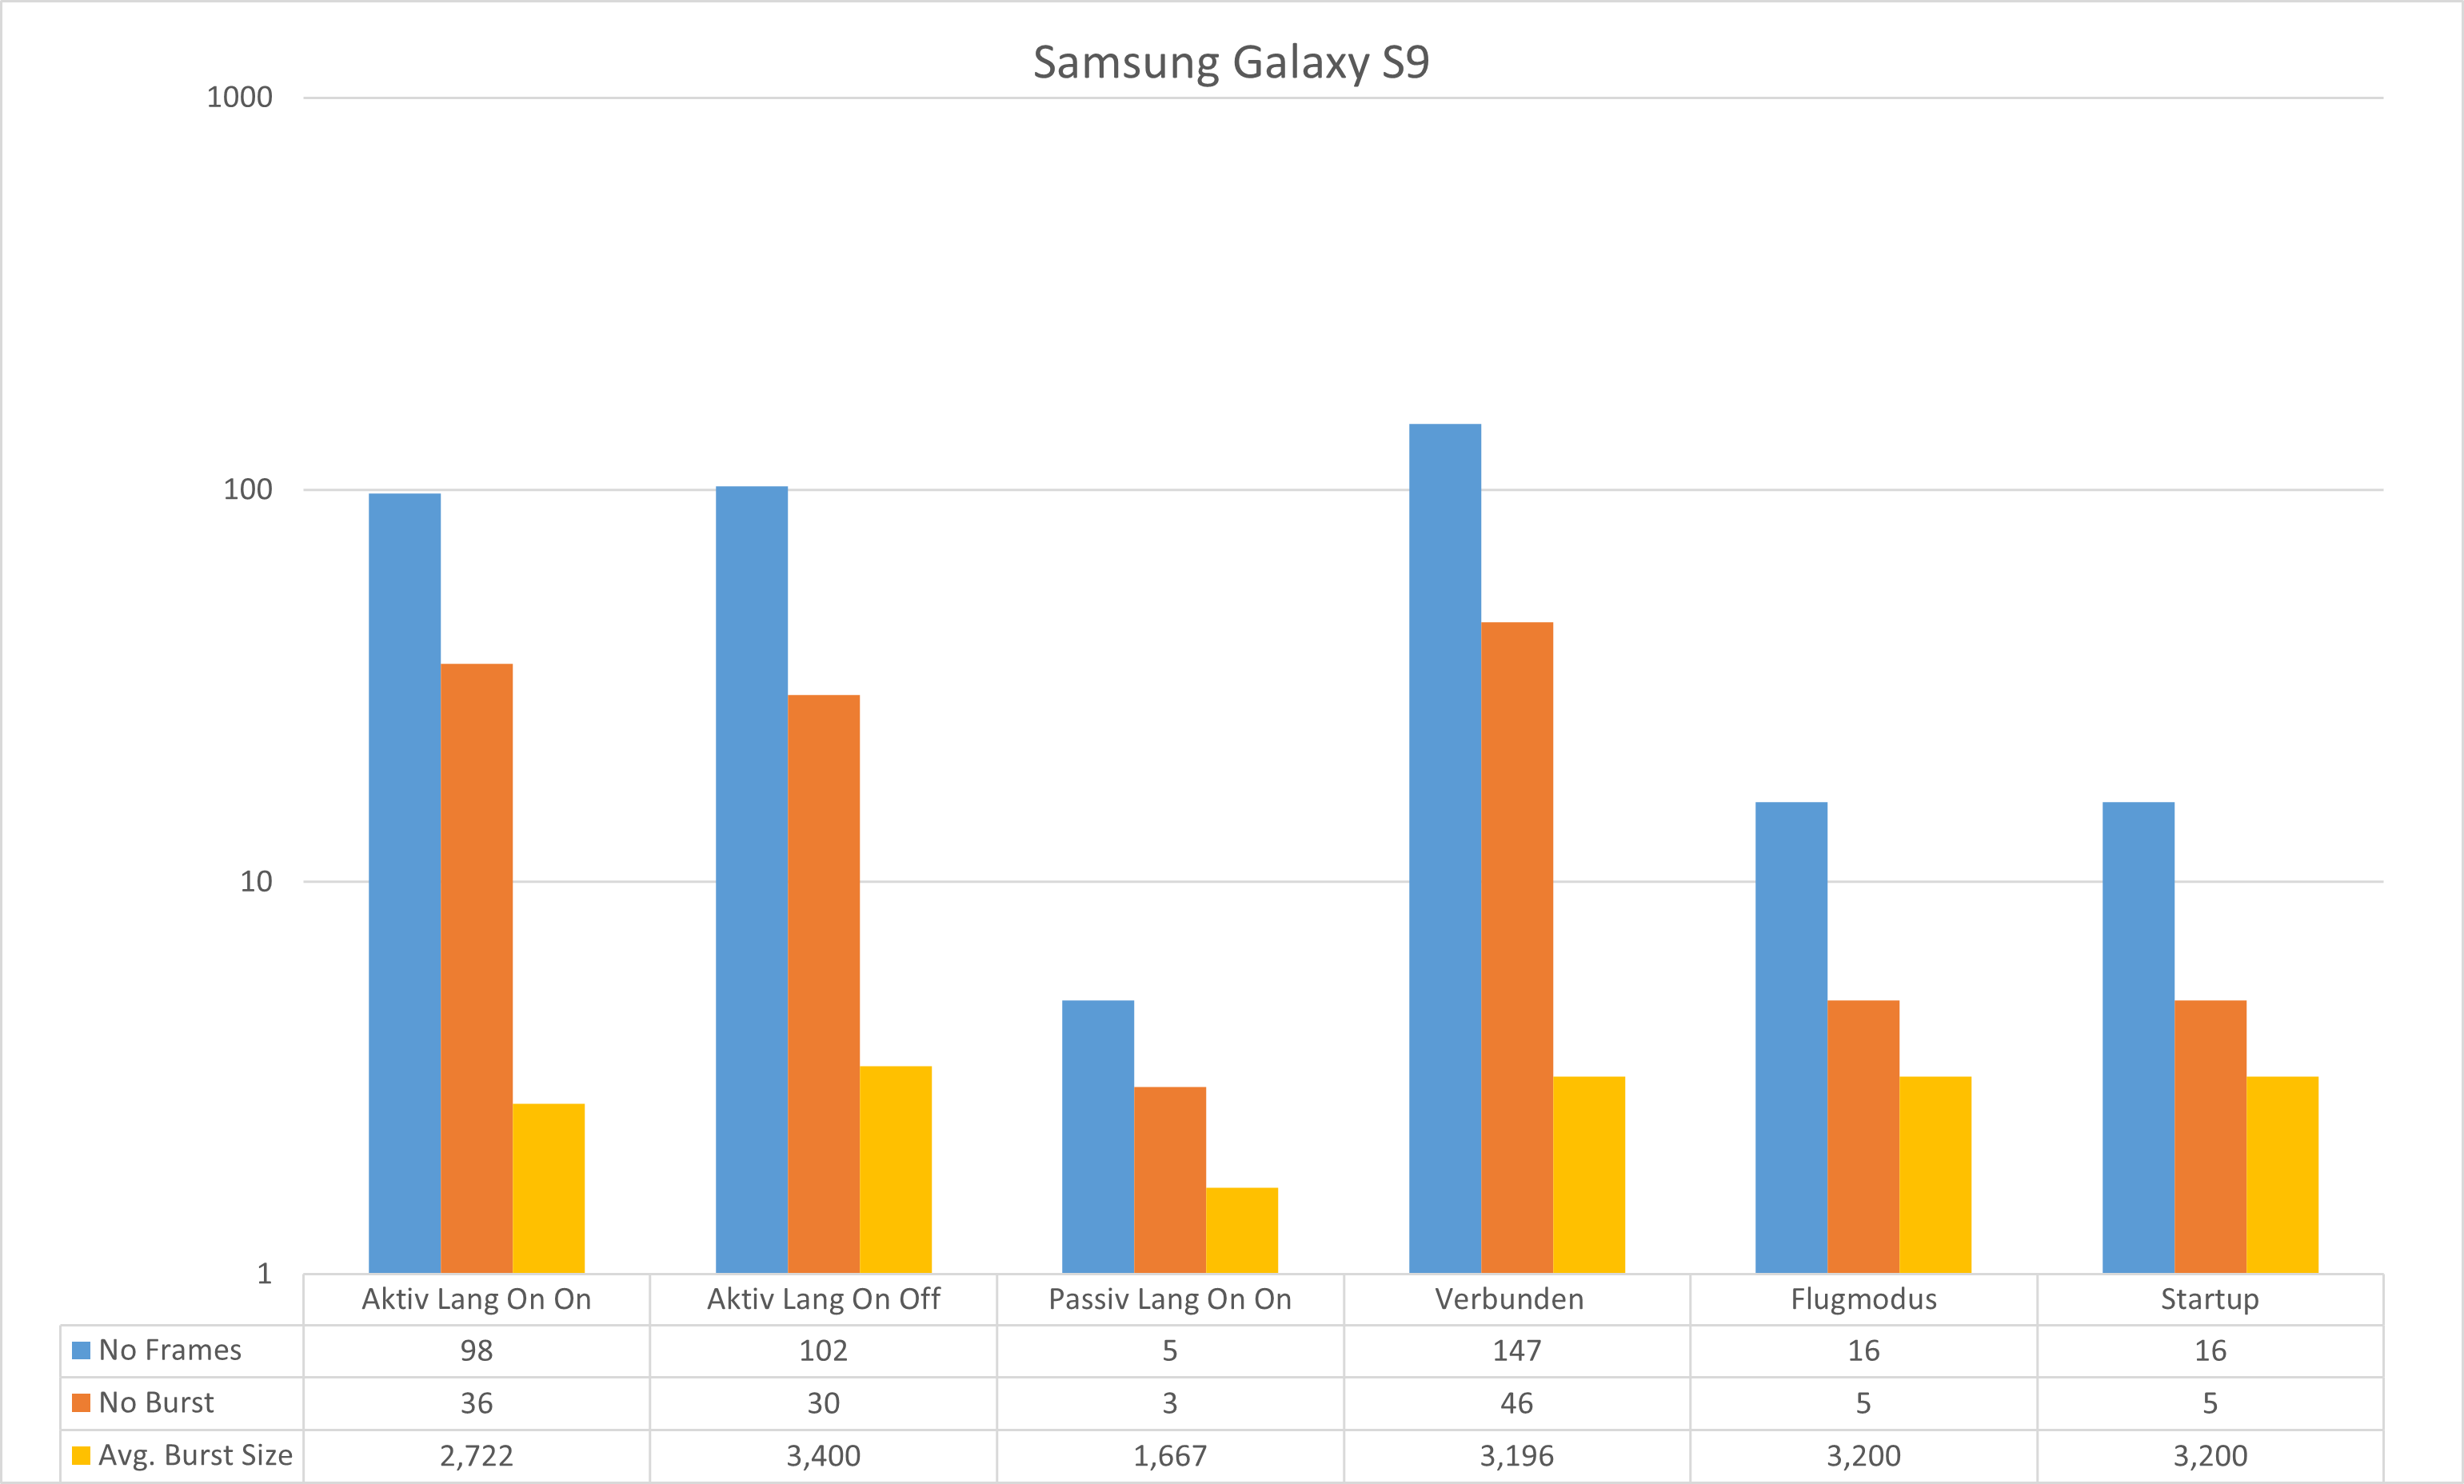
\includegraphics[width=1\linewidth]{Experiments/S9-10.png}
    \caption{Messergebnisse Samsung Galaxy S9 - Android 10}
    \label{figure:androidmeasurementsbycategorys9}
\end{figure}

\begin{figure}[h!]
    \centering
    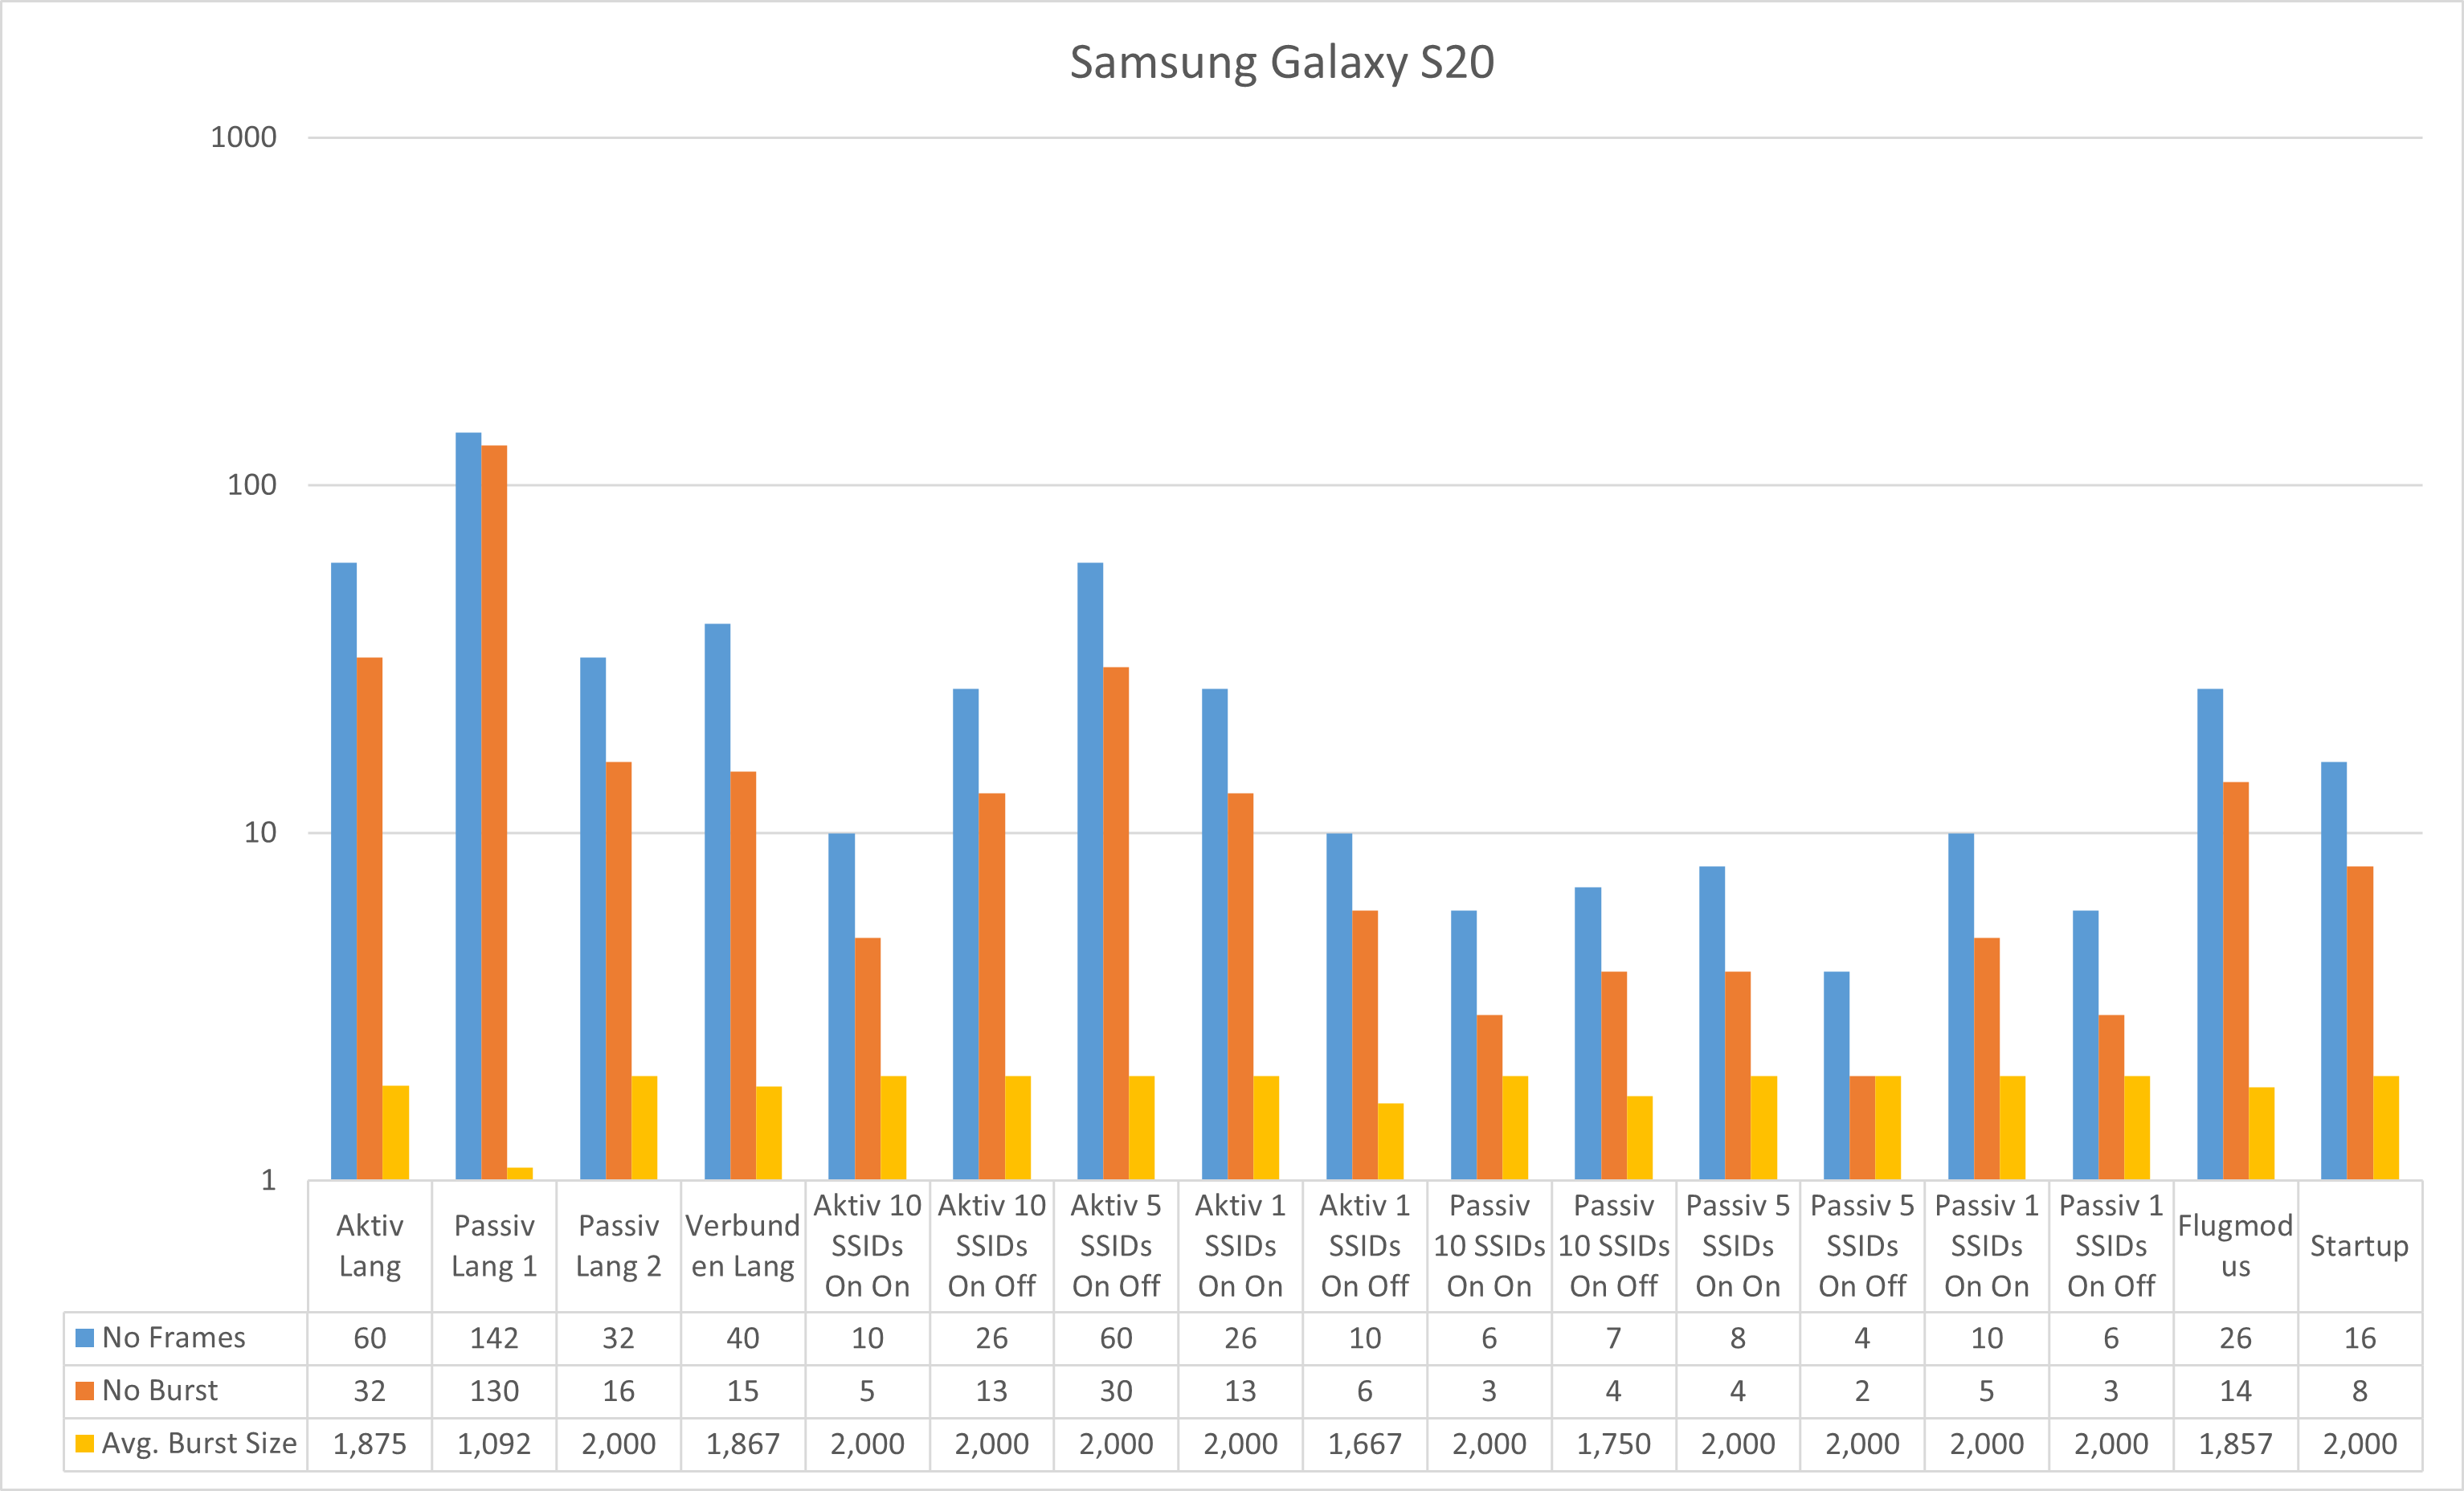
\includegraphics[width=1\linewidth]{Experiments/S20-10.png}
    \caption{Messergebnisse Samsung Galaxy S20 - Android 10}
    \label{figure:androidmeasurementsbycategorys20}
\end{figure}

\clearpage

\begin{figure}[h!]
    \centering
    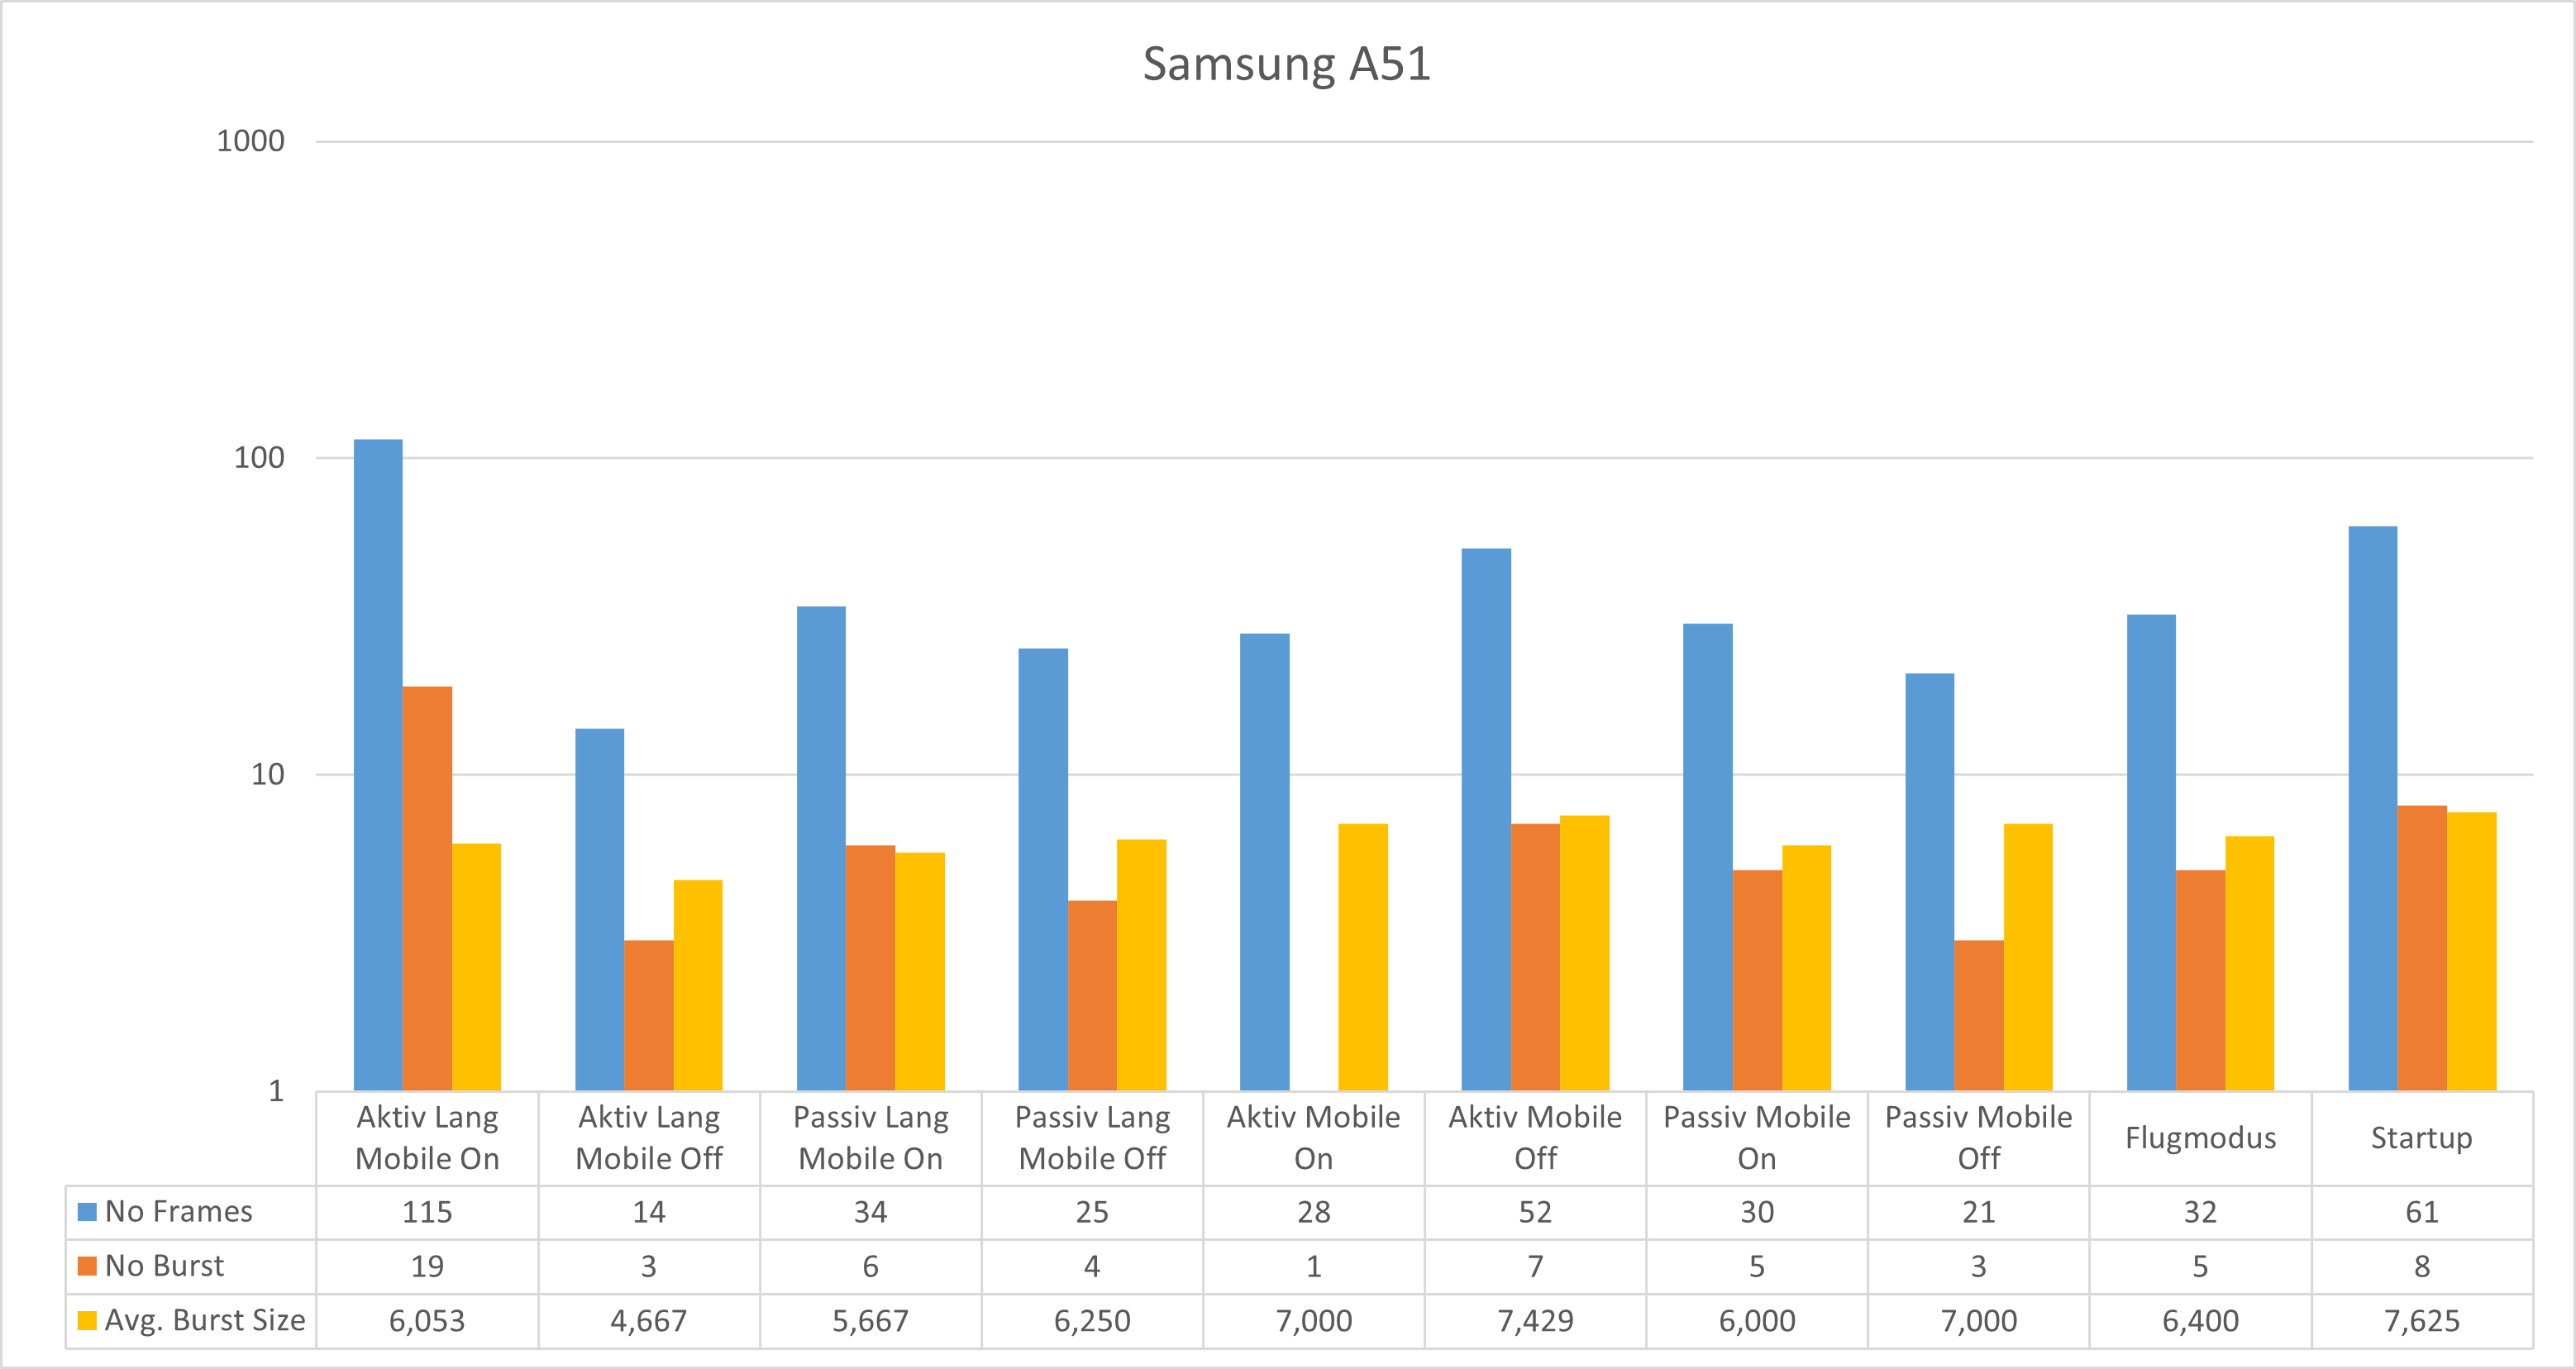
\includegraphics[width=1\linewidth]{Experiments/A51-10.png}
    \caption{Messergebnisse Samsung A51 - Android 10}
    \label{figure:androidmeasurementsbycategorya51}
\end{figure}

Besonders interessant bei der Messung des A51 ist die Tatsache, dass 
das Gerät für alle Messungen immer die MAC-Adresse "02:00:00:00:00:00"
verwendet hat. Lediglich in den Startup- und Flugmodus-Messungen sind 
weitere Probe-Requests mit zufällig generierten MAC-Adressen versendet worden.

\clearpage

\begin{figure}[h!]
    \centering
    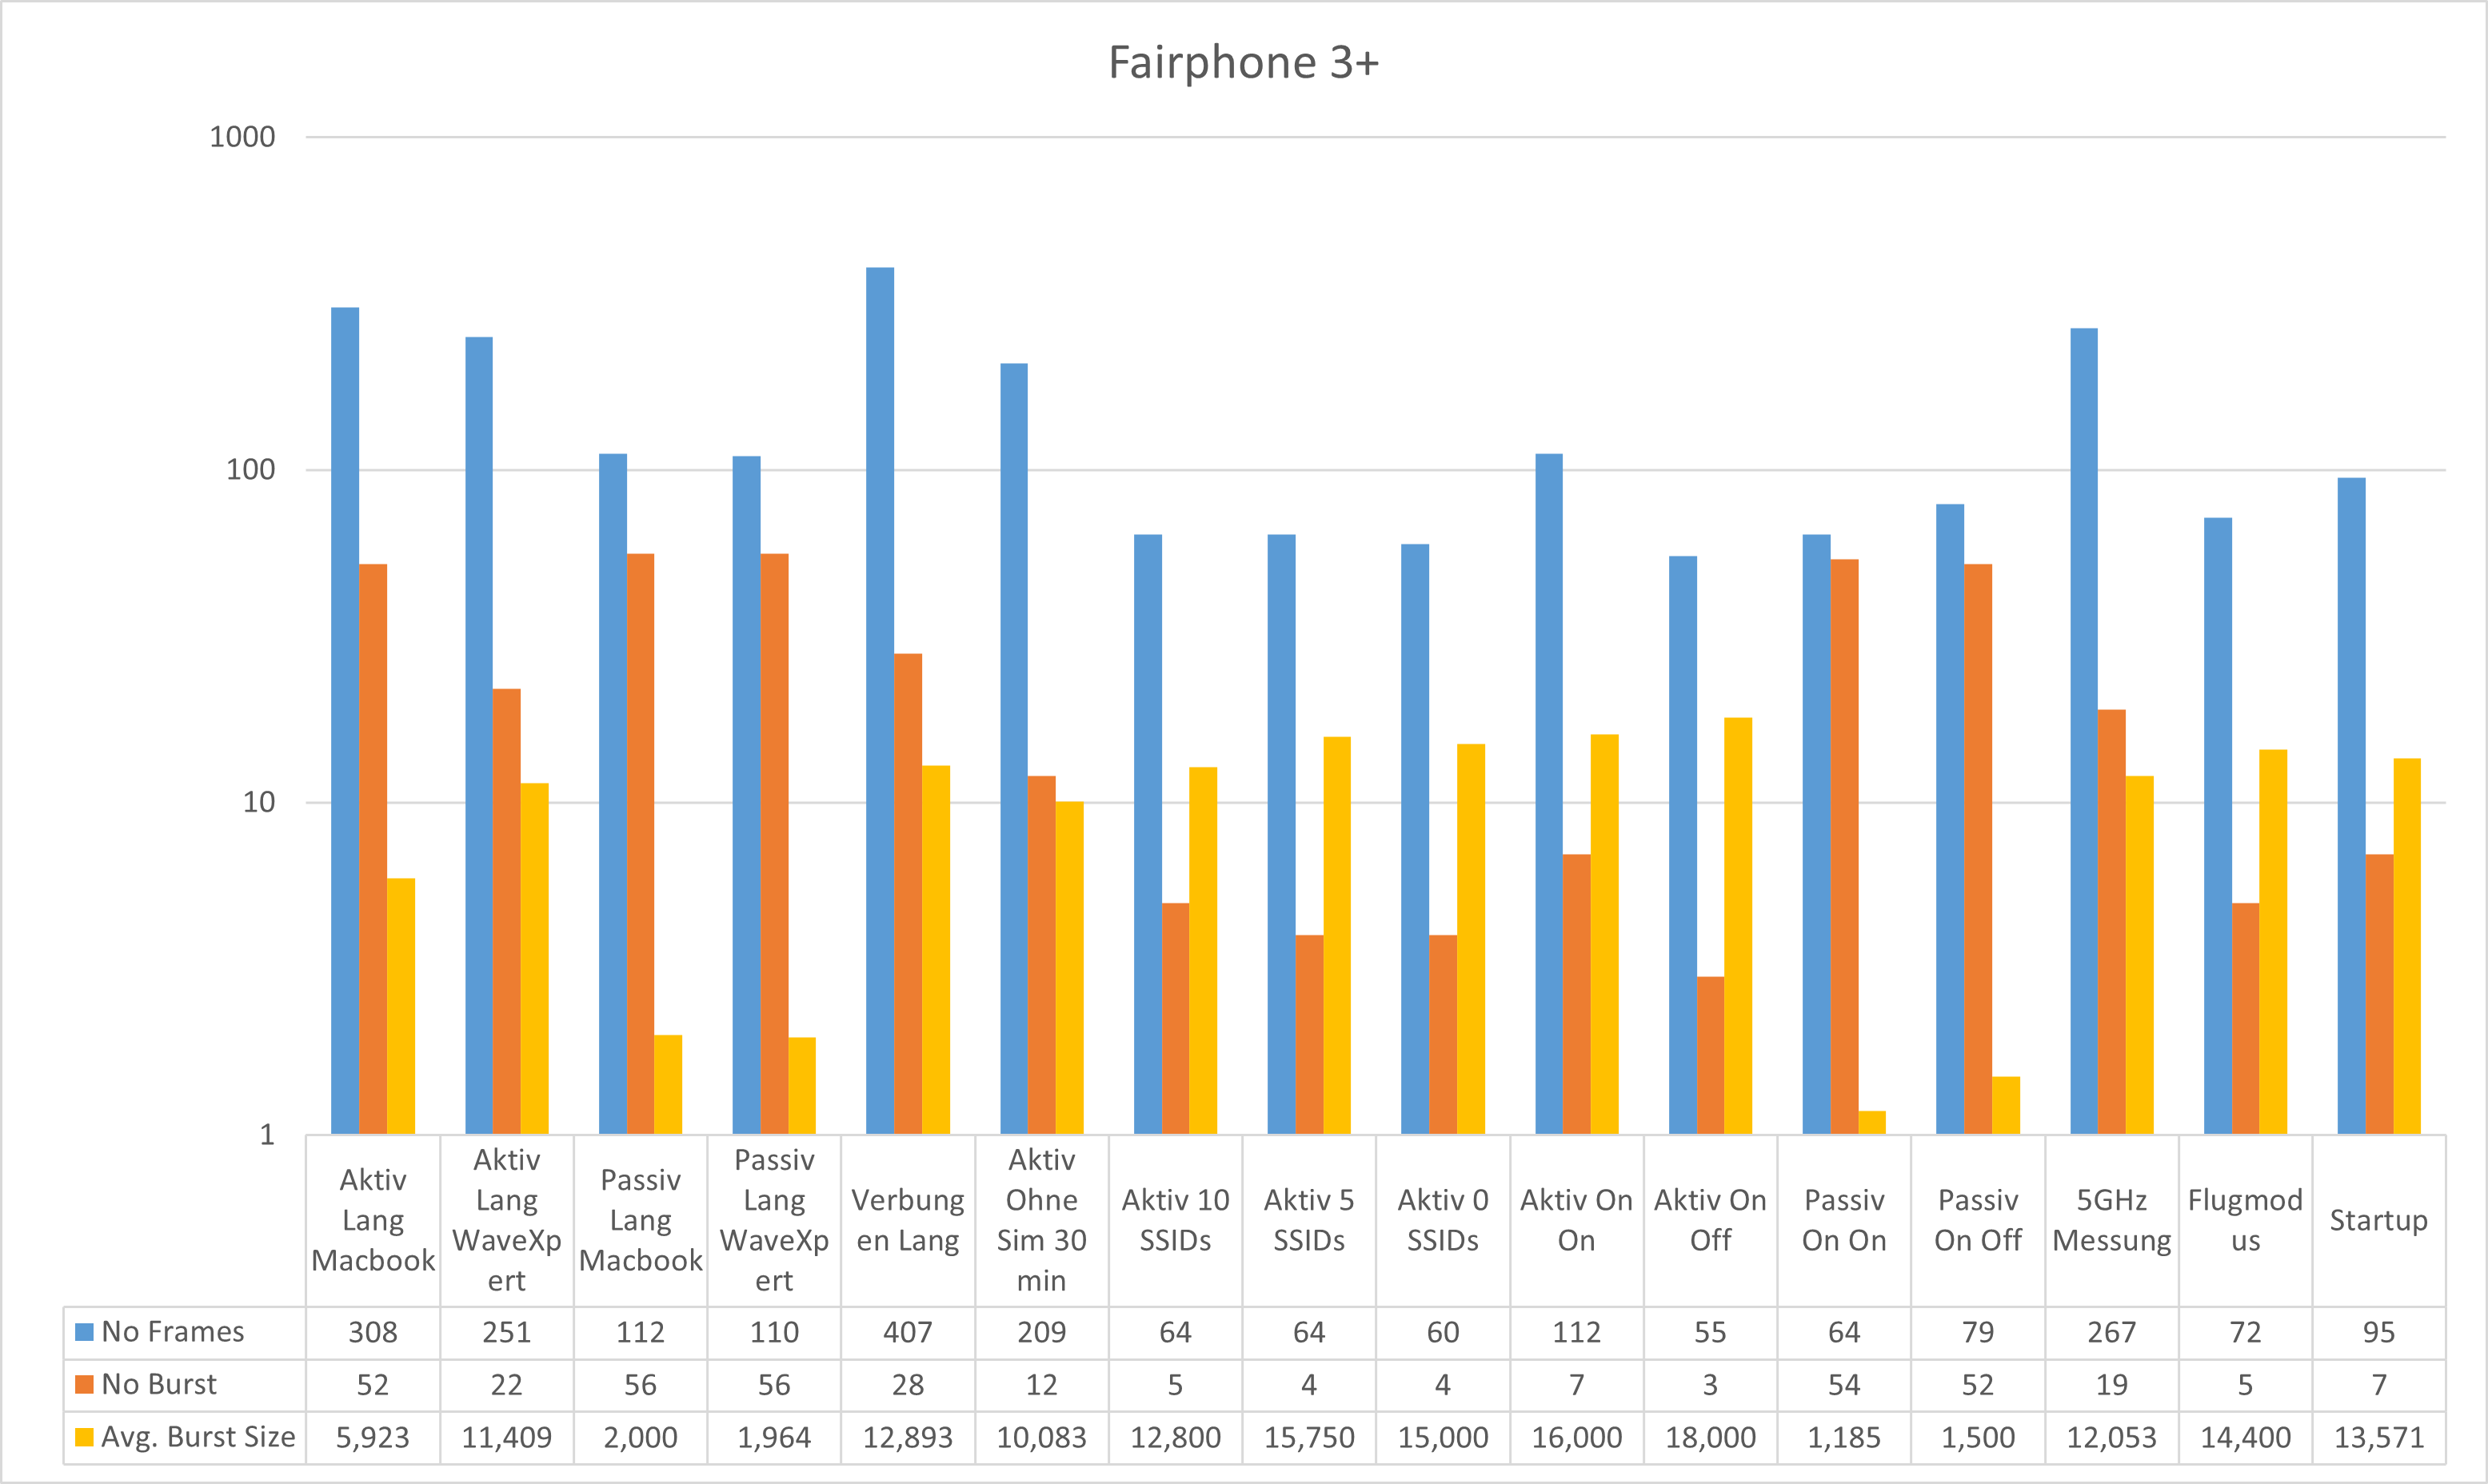
\includegraphics[width=1\linewidth]{Experiments/Fairphone3-10.png}
    \caption{Messergebnisse Fairphone 3+ - Android 10}
    \label{figure:androidmeasurementsbycategoryfairphone}
\end{figure}


Das Fairphone 3+ fällt dadurch auf, dass für die passiven Probe-Requests eine
MAC-Adresse mit Google-OUI und zufälliger NIC verwendet wird. Weiterhin 
ist die Zwischenankunftszeit bei passiven Probe-Request Bursts immer um die 
$63 s$. 

Die Messungen mit dem Fairphone wurden alle mit dem WaveXpert durchgeführt
und es ist in den aufgezeichneten Ergebnissen sehr gut ersichtlich, dass
das Fairphone jeweils einen Burst Probes auf einem Kanal absendet, danach 
den Kanal wechselt und dort die nächste Gruppe Probe-Requests aussendet. 

\begin{figure}[h!]
    \centering
    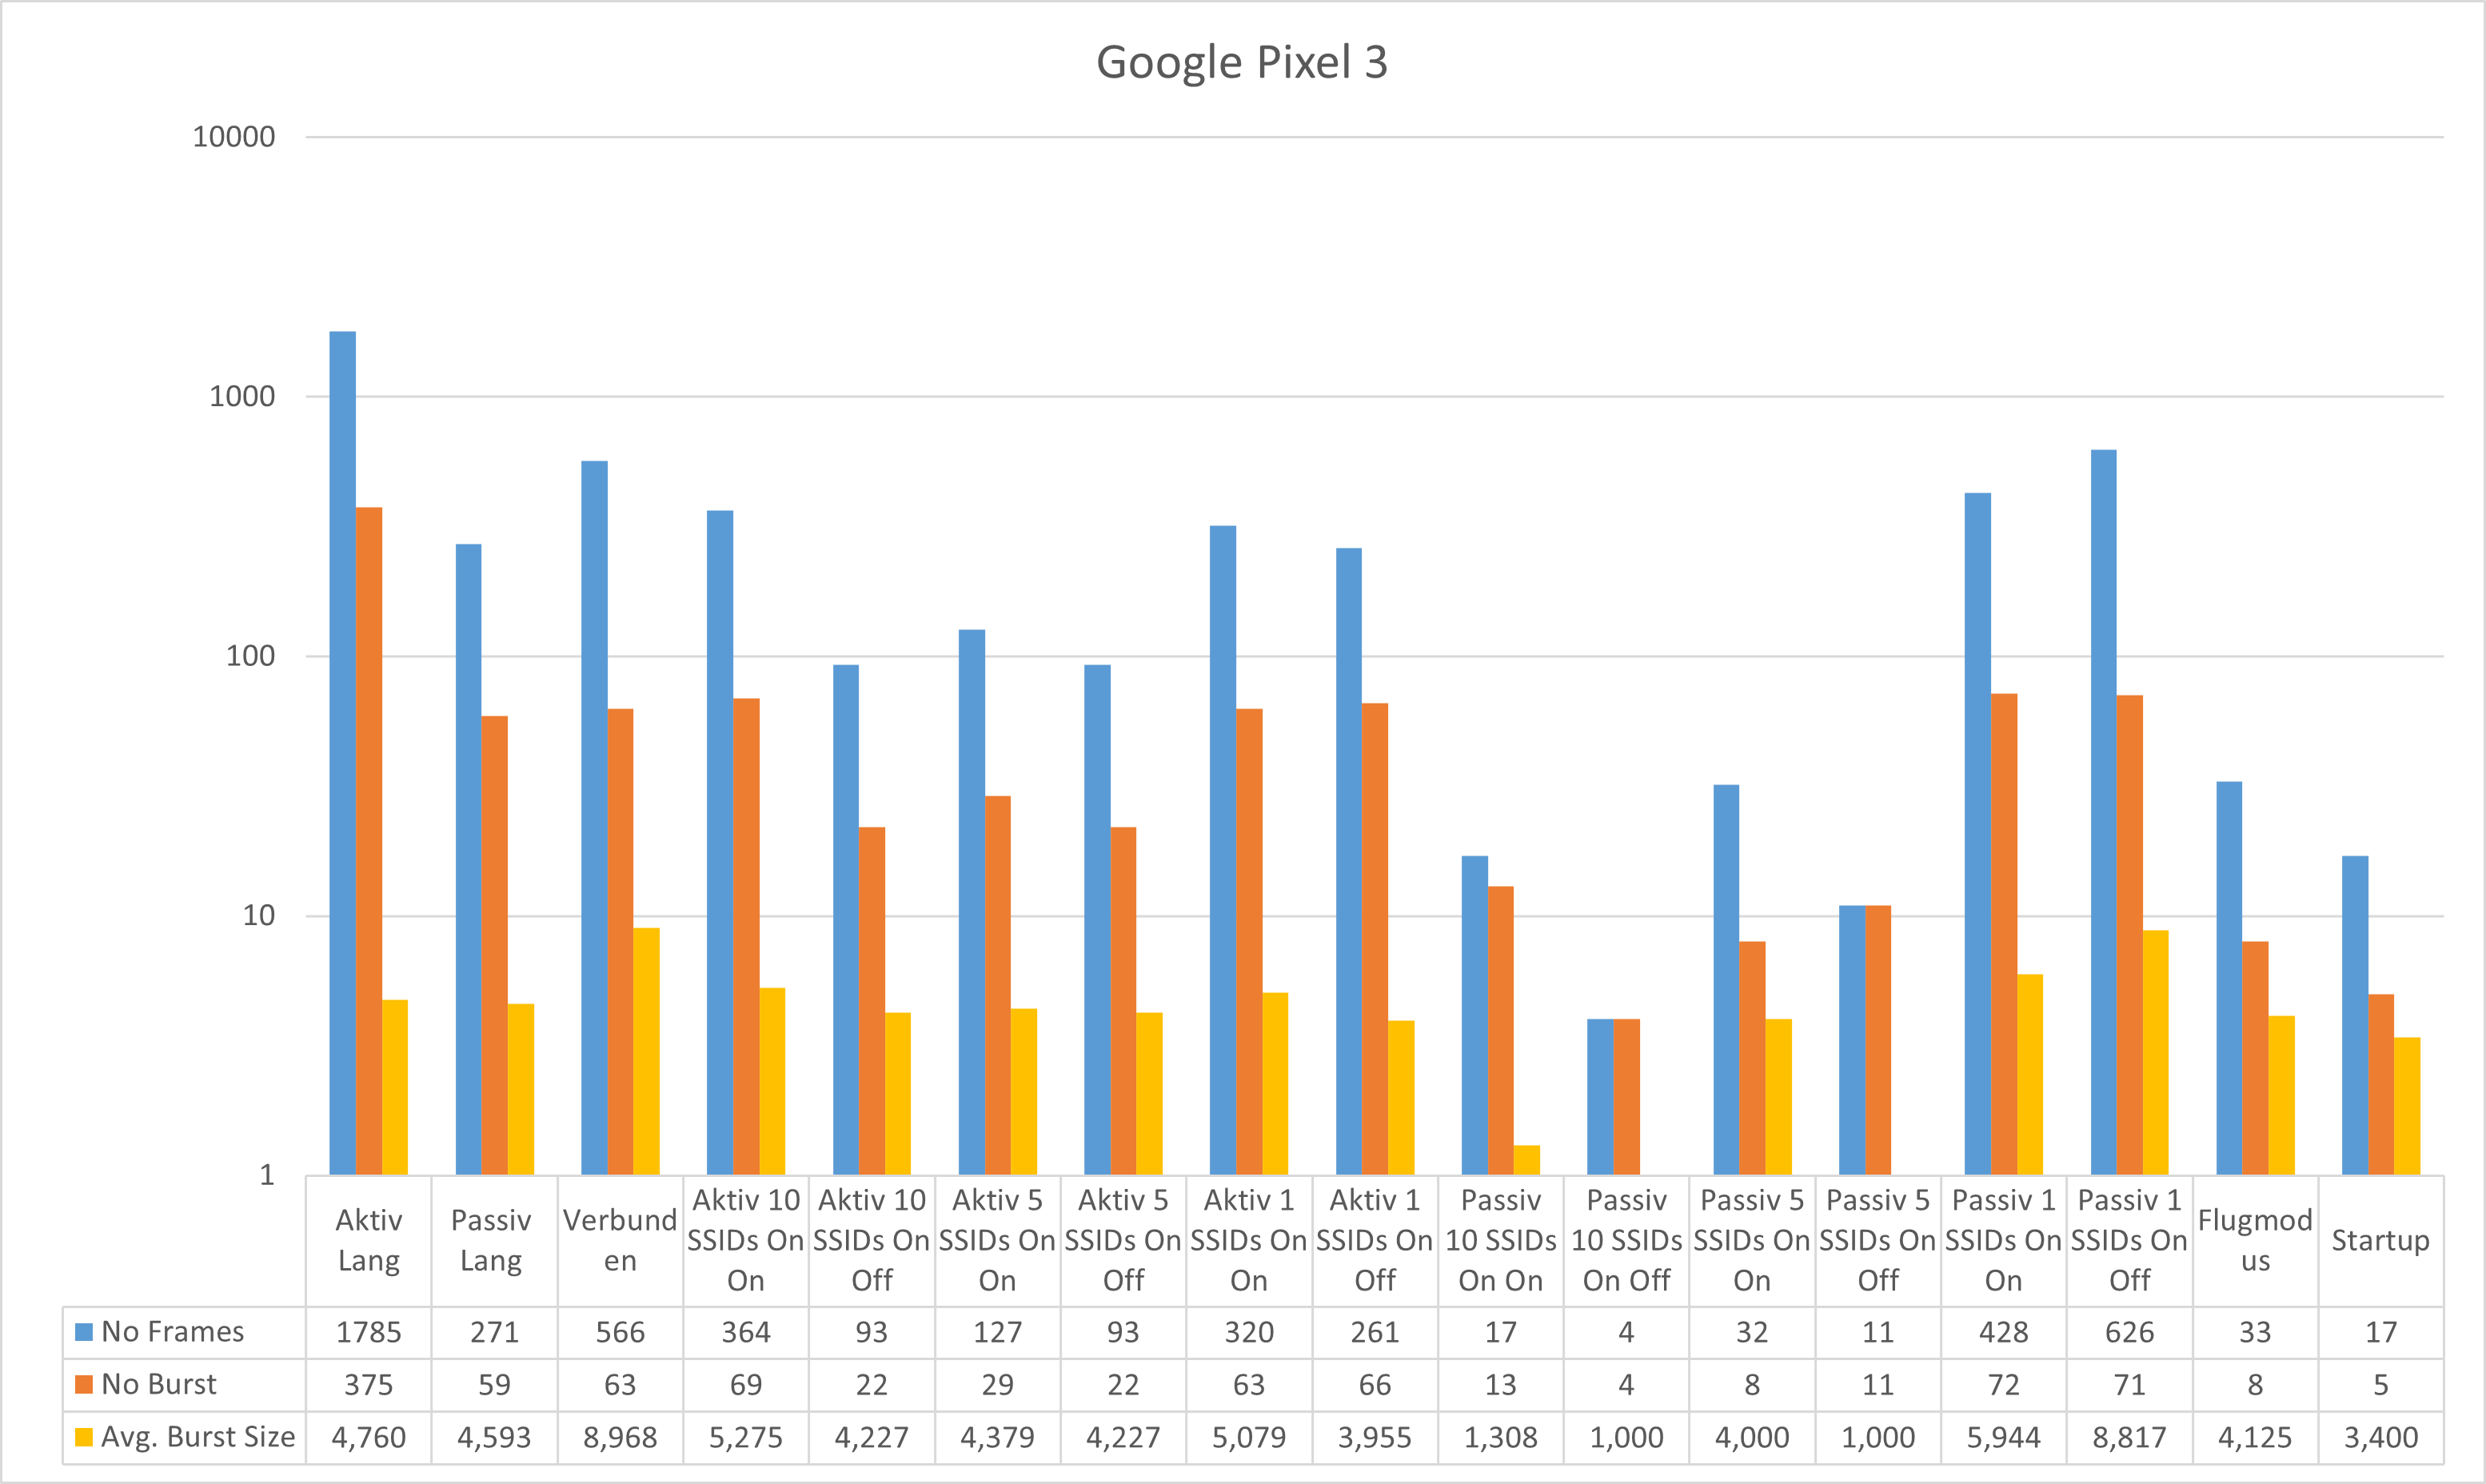
\includegraphics[width=1\linewidth]{Experiments/Pixel3-11.png}
    \caption{Messergebnisse Google Pixel 3 - Android 11}
    \label{figure:androidmeasurementsbycategorypixel}
\end{figure}

\clearpage

\subsubsection*{Erkenntnisse aus den Android-Messungen}
In total $9016$ aufgezeichneten Probe-Requests sind im Schnitt jeweils $5.52$ 
Frames pro Burst mit einer durchschnittlichen Zwischenankunftszeit von $118.24 s$
gemessen worden. Die Bursts beinhalten zwischen einem und 25 Frames.

Mit $4328$ geschätzten verpassten Frames haben Android-Geräte weniger verpasste
Frames relativ zu den aufgezeichneten Frames, was in den Messungen mit dem 
WaveXpert darauf zurückgeführt werden kann, dass Android Geräte die Frames 
pro Kanal gruppiert aussenden. Anders ausgedrückt, ein Android-Gerät sendet 
zuerst einige Frames auf einem Kanal aus, wechselt dann den Kanal und sendet
die nächste Gruppe. Der Vorgang wiederholt sich bei jedem Burst.

Bei genauerer Betrachtung der pcap oder JSON-Dateien zu den einzelnen Messungen
fällt auf, dass Android-Geräte IE-Felder gem. den Tabellen~\ref{table:androidcommoniefields}
und~\ref{table:androidvendorspecificiefields} beinhalten.


\begin{table}[h!]
    \centering
    \begin{tabular}{|c|c|c|c|c|}
        \hline
        \textbf{Tag-NR} & \textbf{0} & \textbf{1} & \textbf{50} & \textbf{3} \\
        \textbf{Tag-Name} & \textbf{SSID} & \textbf{Supported Rates} & \textbf{Ex. Supp. Rates} & \textbf{DS Params Set} \\
        \hline 
        Geräte & alle & alle & alle & alle \\
        \hline
    \end{tabular}
    \caption{IE-Felder, die in allen Messungen vorkommen
    \label{table:androidcommoniefields}}  
\end{table}
Die einzige Ausnahme davon ist das Fairphone 3 welches in den Passivmessungen den 
DS Parameter Set Tag nicht verwendet.

Der in den iOS-Messungen gängige Tag Interworking (107) wird bei Android-Geräten 
nicht verwendet. Dieser Tag kann somit in einem Fingerprinting für die Unterscheidung
von Android- und iOS-Geräten verwendet werden.

Weiterhin verwendet das Google Pixel 3 die HT Capabilities nur im verbundenen Zustand
und die Extended Capabilities gar nicht. Das Fairphone 3 verwendet die Extended Capabilities
auch nie und die HT-Capabilities nur im Passiven Zustand.

\clearpage

\begin{table}[h!]
    \centering
    \begin{tabular}{|c|c|c|c|c|}
        \hline
          & \textbf{Microsoft Corp.} & \textbf{Broadcom} & \textbf{Epigram, Inc} & \textbf{Wi-Fi-Alliance}\\
        \hline 
        A51 & x & & & \\
        Galaxy S8 One & x & x & x & \\
        Galaxy S8 Two & x & x & x & \\
        Galaxy S8 Three & x & x & x & \\
        Galaxy S8 Four & x & x & x & \\
        Galaxy S9 & x & x & x &  \\
        Galaxy S20+ & x & x & x & x \\
        Google Pixel 3 & x & & & x \\
        Fairphone 3+ & x & & & \\ 
        \hline
    \end{tabular}
    \caption{Herstellerspezifische Felder (Vendor Specific - 221)
    \label{table:androidvendorspecificiefields}}  
\end{table}
Auch der Vendor Specific Tag mit der Apple-OUI wird in Android-Geräten nie verwendet
und kann für ein Fingerprinting verwendet werden.

In allen Android Geräten ist das Local Bit gesetzt, was in einem Fingerprinting für eine
zusätzliche Unterscheidung von Android und iOS Geräten genutzt werden kann.

Das Samsung A51, das Fairphone 3+ und die Galaxy S8 haben über mehrere Bursts 
hinweg aufsteigende Sequenznummern.

\subsubsection*{Vergleich mit den MAC-Adressen der Vorarbeit}
In der Vorarbeit wurde eine Tabelle mit den häufigsten auftretenden OUI's von
MAC-Adressen erstellt. Die in dieser Arbeit gemessenen Adressen wurde mit der
Tabelle der Vorarbeit verglichen, um allenfalls Muster zu erkennen. 
Die OUIs der Vorarbeit sind in der Tabelle~\ref{table:commonouis} abgebildet.
CSV-Listen mit den MAC-Adressen aus den Messungen sind im Repository im 
Ordner "Experimente" zu finden.

Es wurden keine Übereinstimmungen der MAC-Adressen aus den Messungen mit den 
OUIs der Vorarbeit gefunden.

\clearpage